\section{Intents, Cover and Order Relation Generation}\label{sec:intent-generation}

Our initial design for the intent prediction was split into 3 modules:
\begin{enumerate}
    \item the first module would create a skeleton for the intents, from the concept number upper bound and the attribute embeddings;
    \item the second module would predict the intents, from the skeleton and the object and attribute embeddings;
    \item the last module would use the intents and the attribute embeddings to predict the links; this last module wouldn't share its gradient with the first two.
\end{enumerate}

Experimental results led us to simplify the model by merging the 3 modules into a simpler model described in \cref{fig:fcat}.
The resulting architecture relies on a DAN, an LSTM, and attention mechanisms described in the next paragraphs.
The DAN takes the attribute embeddings as input, and generates a single output per FC which is then used at every step of the generation process, as shown in \cref{fig:fcat}.
We expect it to learn general information about the FC similarly to how the number of concept prediction works.
In addition to the output of the DAN and the attention contexts, the LSTM is fed the number of concept upper bound and the index of the current intent.

\begin{figure}
    \centering
    \subcaptionbox{Concept generator at step $k$}{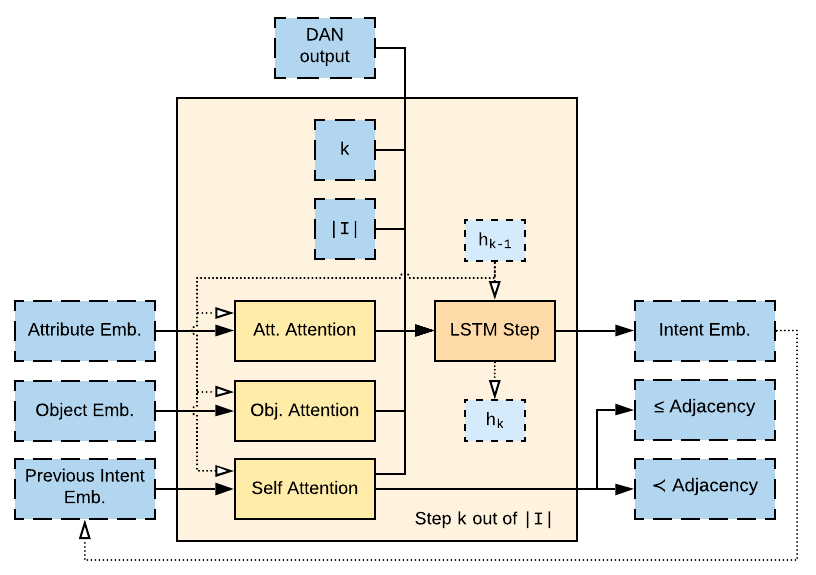
\includegraphics[keepaspectratio, height=5cm, width=.48\textwidth]{Figures/Ch3/fcat_cell.png}}
    \subcaptionbox{Full architecture}{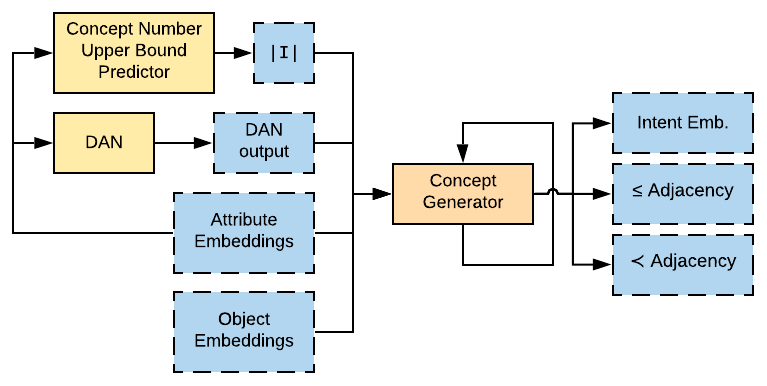
\includegraphics[keepaspectratio, height=5cm, width=.48\textwidth]{Figures/Ch3/fcat_full.png}}
    \caption{Schematic representation of the intent generation architecture. Blue blocks correspond to tensors and orange to neural components.}
    \label{fig:fcat}
\end{figure}

For intent generation we use a basic version of attention, equipped with multiple attention heads.
Attention heads can be seen as reading heads scanning the same sequence, but each head performing a different scan.
Our attention mechanism works by comparing a query $q$ with sequence $S$ of elements.
The query at step $k$ of the generation is obtained by flattening the hidden state generated at step $k-1$.

Let $\varphi$ be a feed-forward layer with input and output size $|s|$ for $s\in S$.
Let $\psi_i$ be a feed-forward layer associated with head $i$ with input size $|q|$ and output size $|s|$.
Finally, let $\cdot$ be the dot product.
The attention weight computed by head $i$ for element $s$ can be expressed as $weight_i(s,q) = \varphi(s) \cdot \psi_i(q)$.
A softmax is applied to all the weights of an head, which are then used to compute the attention summary $summary_i(S,q) = \sum_{s\in S} softmaxedWeight_i(s,q) \times \varphi(s)$.
We also use a sigmoid variant of our attention for which the weights are $weight_i(s,q) = sigmoid(\varphi(s) \cdot \psi_i(q))$.

In our model we use 3 attentions, each equipped with 4 heads, for a total of 12 attention heads:\begin{itemize}
    \item an \textit{object attention}, an attention applied on the set of object embeddings;
    \item an \textit{attribute attention}, an attention applied on the set of attribute embeddings;
    \item a \textit{self attention}, an attention applied on the previously generated intents.
\end{itemize}
Two of the self attention heads are of the sigmoid variant, and are used to predict the relations between the currently seen intent (or concept) and the attended intent (or concept). The sigmoid attention weight serve as a probability of there being an edge between the current concept and the previous one, \textit{à la} GraphRNN.
One of the heads is dedicated to $\leq$ and the other to $\prec$.

Compared to our preliminary experiments, the soft attention is split in two because there are two input sequences, and the link attention correspond to the two sigmoid attention heads of the self attention.


